The two layers surveyed so far are usually discussed as independent engineering problems. They are not: both place requirements on the same runtime state, and those requirements pull in opposite directions. Diagnostics needs state to be \emph{retained} long enough to explain a failure; serving infrastructure needs it \emph{discarded} quickly enough to serve the next request. The organising axis is therefore \emph{retention}, not timing: serving systems choose a retention policy with no regard for what diagnosis will need, and diagnosis, online or after the fact, must work from whatever survives. By the time an explanation is produced the discarded state is already gone, so the question is what the policy kept, not when the diagnosis ran.

The clearest evidence is a measurement rather than an argument. TraceElephant reports the same attribution task under two observability settings, and the gap is large: under the All-at-Once protocol, complete traces raise agent-level accuracy from 51\% to 62.2\%, and step-level accuracy from 16\% to 28.1\% (a 76\% relative gain)~\citep{traceelephant2026}. Output-only traces are not a failure of instrumentation; they are what a cheap-capture policy produces, because capturing every observation at every step is expensive to store and ship. That measured 76\% relative drop in step-level attribution is therefore the price of a retention decision, and it is a diagnostic cost no serving system currently accounts for.

\begin{figure*}[t]
\centering
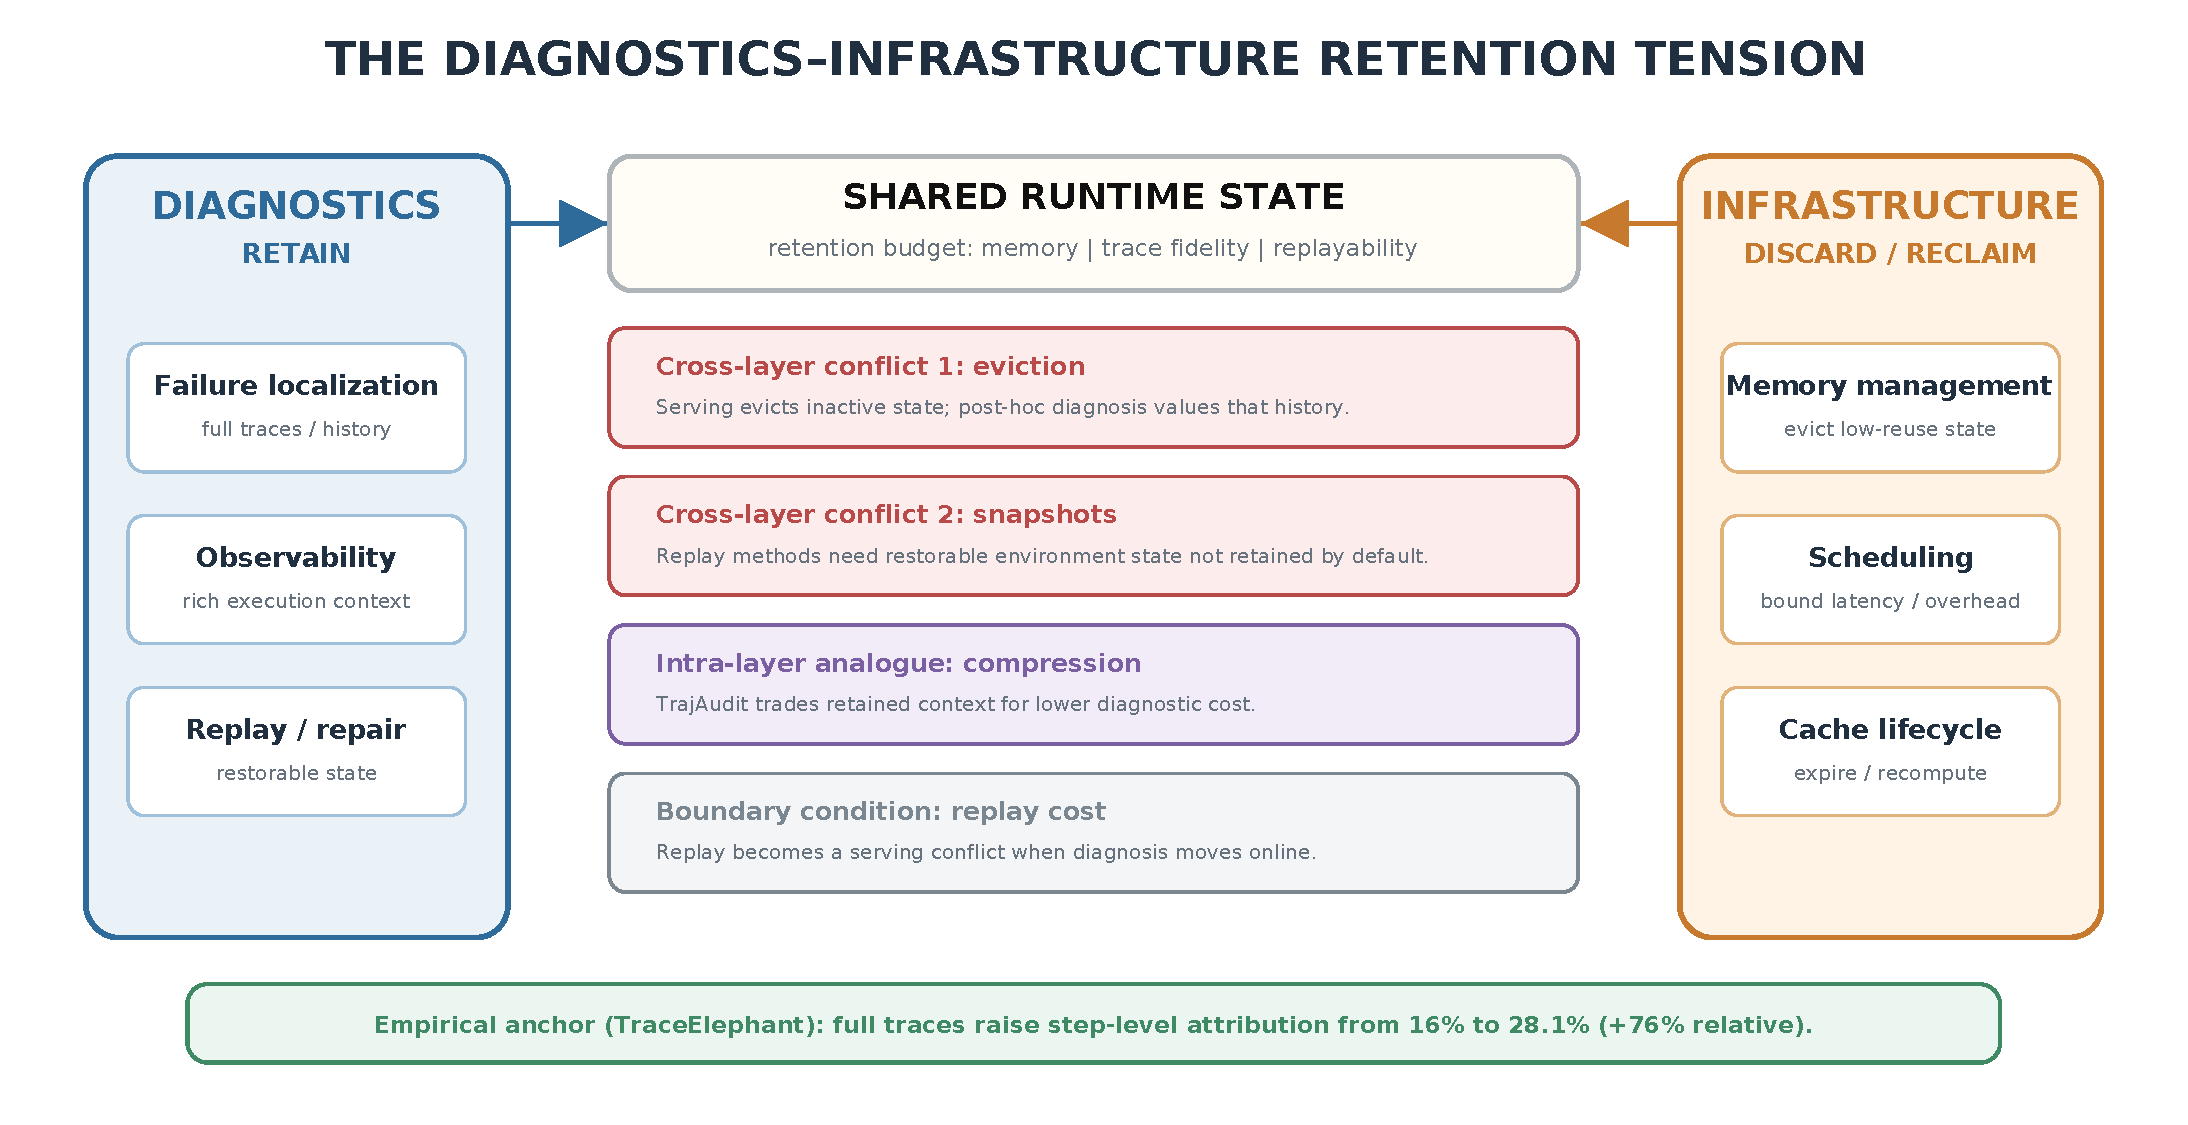
\includegraphics[width=\textwidth]{fig5_tension.pdf}
\caption{The diagnostics--infrastructure retention tension. The diagnostics layer (left) requires runtime state to be \emph{retained} for failure explanation, while the infrastructure layer (right) requires it to be \emph{discarded} for fast service. Two cross-layer conflict mechanisms, one intra-layer analogue, and one boundary condition act on shared runtime objects (centre). No existing system manages the retention budget as a first-class resource.}
\label{fig:tension}
\end{figure*}

We call this the diagnostics--infrastructure retention tension. It is not merely a matter of engineering effort left undone: the two layers optimise against different objectives on the same resource, so a policy that is optimal for one is close to anti-optimal for the other. Two cross-layer mechanisms make the conflict concrete; a third instance shows the same shape within the diagnostic layer itself; and a fourth marks where the conflict would become acute for online diagnosis.

\emph{Swapping state off the fast path.} ScaleSim's distance-aware eviction~\citep{zhou2026} selects the agent states with the longest invocation distance and moves them out of GPU memory, which is, from the diagnostics side, the set of inactive agents whose state a post-hoc attribution method would need in order to reconstruct the failure. The serving engine does not delete this state; it swaps it to host memory or storage. The retention question is therefore not whether the swap happens but whether the swapped-out state is reclaimed before diagnosis reads it, and whether the KV-cache is preserved or dropped and recomputed. A policy that is optimal under a memory budget makes the diagnostic copy the first candidate for reclamation, which is the conflict in its precise form.

\emph{Environment snapshots are not retained.} Replay-based attribution needs more than a text trace. FAMAS~\citep{famas2025} re-executes a failed task $k=20$ times and expects the environment to reach comparable states, and DoVer~\citep{dover2026} intervenes mid-trajectory and reruns from the intervention point, which requires the environment to be restorable. Serving infrastructure has no reason to retain environment snapshots, since they are not needed to schedule the next request. This is the concrete resource the replay-class methods lack, and it explains why they are evaluated on fixed corpora where the environment can be reconstructed offline rather than on live serving paths.

\emph{The diagnostic layer has an isomorphic tradeoff internally.} TrajAudit's Semantic Saliency Folding~\citep{trajaudit2026} compresses 86--92\% of observations into placeholders to fit the model's context window. This is the diagnostician's own retention decision, with more context yielding better attribution and less yielding lower cost. It is not cross-layer tension but a same-shaped problem inside one layer, and we note it because it shows the accounting question is not specific to serving.

\emph{Replay is a serving cost: a boundary condition.} The boundary flagged here is the replay budget itself, which is a separate concern from the restorable environment the previous instance requires: a method could hold a restorable environment and still replay once. FAMAS's twenty replays conflict with serving only if diagnosis runs on the serving path. FAMAS is an offline method evaluated on a fixed corpus, so for this instance the conflict is latent rather than actual: it marks where the tension would become acute, namely for any diagnostic that must run online. We therefore treat replay as the boundary condition of the retention argument rather than as a fourth mechanism. The existence of zero-replay debugging~\citep{zeroreplay2026} is indirect evidence that the cost is real when diagnosis is placed on the serving path.

Table~\ref{tab:tension} contrasts the two layers along the dimensions that generate these conflicts. The rows are not independent: retention budget is the shared resource, and every mechanism above is a different way of spending it. No surveyed system treats retention as a managed quantity, and the four co-design directions that follow from this view are developed in \S\ref{sec:discussion}.

\begin{table*}[t]
\centering
\caption{The diagnostics--infrastructure tension along shared runtime resources.}
\label{tab:tension}
\footnotesize
\setlength{\tabcolsep}{5pt}
\begin{tabular}{@{}p{0.20\textwidth}p{0.34\textwidth}p{0.34\textwidth}@{}}
\toprule
\textbf{Dimension} & \textbf{Diagnostics requirement} & \textbf{Infrastructure requirement} \\
\midrule
Runtime state & Full per-step inputs, outputs, and tool logs & Only what is needed to schedule the next request \\
Retention horizon & Retain until diagnosis completes & Discard as soon as reuse probability drops \\
Eviction criterion & Keep low-reuse-probability states & Evict low-reuse-probability states first \\
Granularity & Step-level and cross-agent (to localise cause) & Request- and agent-level (to place work) \\
Overhead budget & Tolerates replay and rich capture & Bounded by serving SLO; overhead is waste \\
Replay resources & Restorable environment snapshots & None retained \\
\bottomrule
\end{tabular}
\end{table*}
\vspace{-2pt}
{\footnotesize \emph{Observed instances.} Cross-layer: ScaleSim's eviction swaps (not deletes) the state a later diagnosis would need~\citep{zhou2026}; serving retains no environment snapshots needed by replay-based attribution~\citep{famas2025,dover2026}. Intra-layer analogue: TrajAudit compresses 86--92\% of observations~\citep{trajaudit2026}. Boundary: replay ($k{=}20$) is affordable only offline~\citep{famas2025}. Continuum's TTL expiry~\citep{continuum2025} raises resumption cost within the cache layer, not across the diagnostics--infrastructure boundary. Output-only capture costs 76\% relative step-level attribution accuracy~\citep{traceelephant2026}.}